\subsection{Creating and Using the \acrshort{ast}}\label{CreatingAst}

The goal for the \acrshort{ast} was to decrease the information in the tree, while making fields on the classes for easier access to the information.
Another way could be having all the nodes connected as children on the tree, but instead of running through the trees children, and looking for specific children, the compiler instead directly access different fields on the nodes instead.
All the nodes of the \acrshort{ast} have been designed with this in mind.
For example on figure \myref{image:ASTDecl} a class structure can be seen, which consists of all the classes needed to express a declaration on the tree.
To use a previous example a declaration could be \texttt{int a = 5;}.

\begin{figure}[!ht]
\centering
 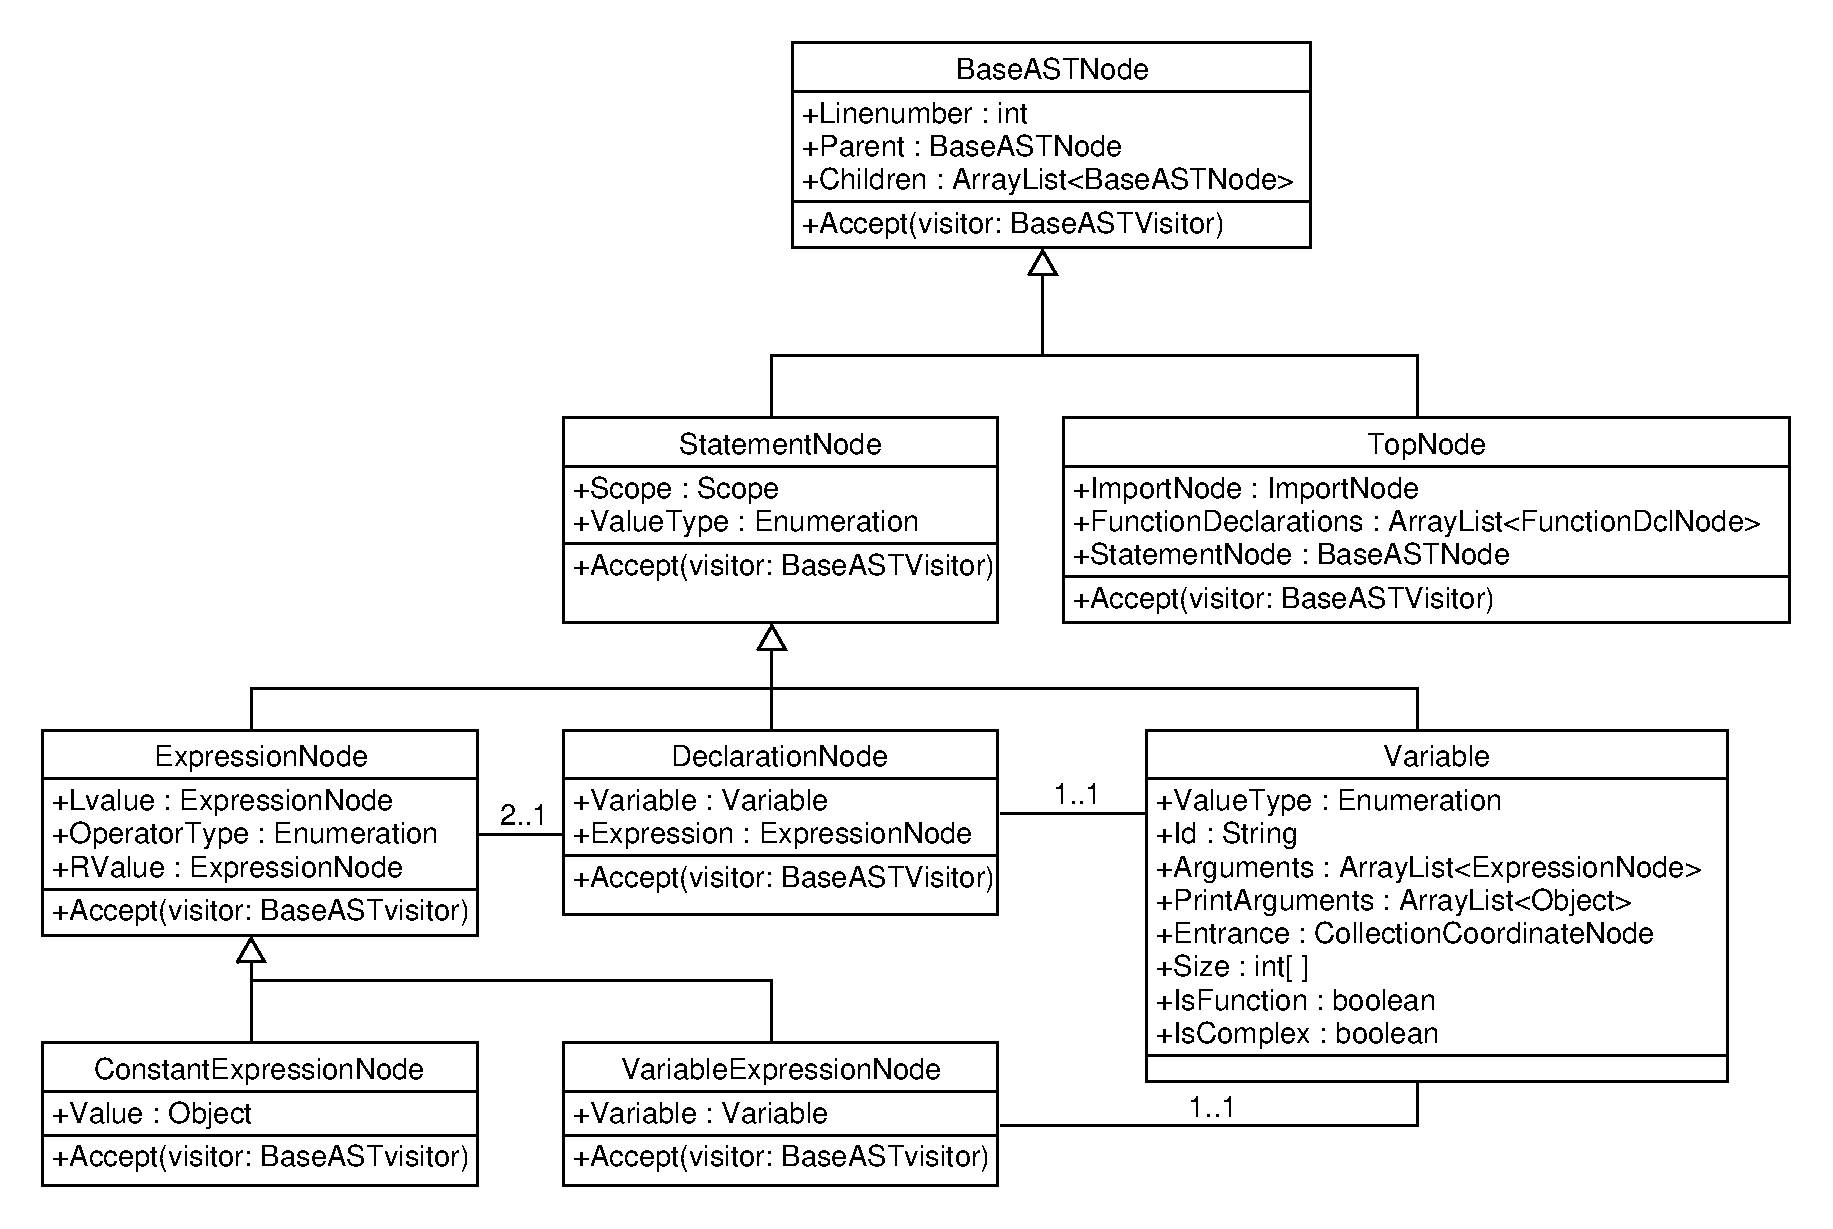
\includegraphics[width=1\textwidth]{figures/ClassDiagrams/ASTDeclarationNodeMoreInfo.pdf} % trim=4.85cm 15cm 0.85cm 1cm
\caption{A UML class diagram of the classes used for a DeclarationNode on the \acrshort{ast}.}\label{image:ASTDecl}
\vspace{-15pt}
\end{figure}

This class contains a lot of different information which is used depending on which class the instance of the \texttt{Variable} is connected to.
If \texttt{Variable} is connected to a VariableExpressionNode, the only fields used on the variable class is ValueType and Id, while the booleans IsFunction and IsComplex are set to false.
But in the example \texttt{int a = 5;} the tree structure looks like the AST on \myref{image:AST}.
If \texttt{Variable} is used when a function is on the right side of an assignment or declaration, an example being \texttt{int a = foo(5);} the fields used on \texttt{Variable} are Id, ValueType, arguments, and the boolean IsFunction is instead set to true.
The printargument field is used when the a functioncall to \texttt{Print();}is made, and entrance, size and IsComplex is used when dealing with the complex types, vectors and matrices.
\texttt{TopNode} sets the structure of a \gls{gamble} program as described in \myref{subsec:Struc}.
The full Classdiagram can be seen in \myref{ASTNodes}.

The classes have made it easier to make a logical traversal of the tree based upon the names of the fields on the classes.
E.g. the \texttt{ForLoopNode} has fields named \texttt{Body}, \texttt{Initialize}, \texttt{Update}, and \texttt{Conditional}, these names has meaning instead of just being children on the node.

The Class \texttt{VisitorAST} creates the \acrshort{ast} from the parse tree, it traverses the tree using the visitor pattern and on every node fills out a the fields of one of the classes for the \acrshort{ast}, and then afterwards the node is placed on the tree as a leaf or field on the node which made the visit call.

One of these visit methods can be seen on \myref{lst:VisitorASTCode}

\begin{lstlisting}[caption=The Visit Method for WhileLoopNode,frame=tlrb,label={lst:VisitorASTCode}]
public BaseASTNode visitWhileLoop(ourLangParser.WhileLoopContext ctx) {
    WhileLoopNode whileLoopNode = new WhileLoopNode(parentStack.peek());
    whileLoopNode.setCondNode(
    	(ConditionalExpressionNode)visit(ctx.conditionalExpression()));
    parentStack.push(whileLoopNode);
    visitChildren(ctx.whileBlock);
    parentStack.pop();
    whileLoopNode.setLineNumber(ctx.start.getLine());
    return whileLoopNode;
}
\end{lstlisting}
A stack called the parentstack is used to keep track of the caller to \texttt{visit()}, in order to keep track of the parents and the children of the tree.
On line 3-4 a call to visit the conditionalexpression of the whileloop is made, which returns an instance of the class \texttt{ConditionalExpressionNode}.
Afterwards, to set the body of the \texttt{WhileLoopNode}, all the children of the nodes are visited, but first the \texttt{WhileLoopNode} is pushed to the parentstack.
This makes it possible to check which node is the parent of the children being created during the calls to visit.

For implementing the Visitor pattern for the \acrshort{ast} an interface was made, which contains a visit method for every single class of the \acrshort{ast}.
A baseclass has then been made which implements this interface.
This baseclass implements each visit method to visit the correct fields of the node in the correct order.
This means that any visitor class only have to override the visit methods which are of interest for the specific visitor.
An UML diagram has been made to show the implementations of the visitor pattern in the compiler and can be seen on \myref{image:Visitors}.
The figure shows how every visitor class inherits from the \texttt{BaseASTVisitor} class.

\begin{figure}[!ht]
\centering
 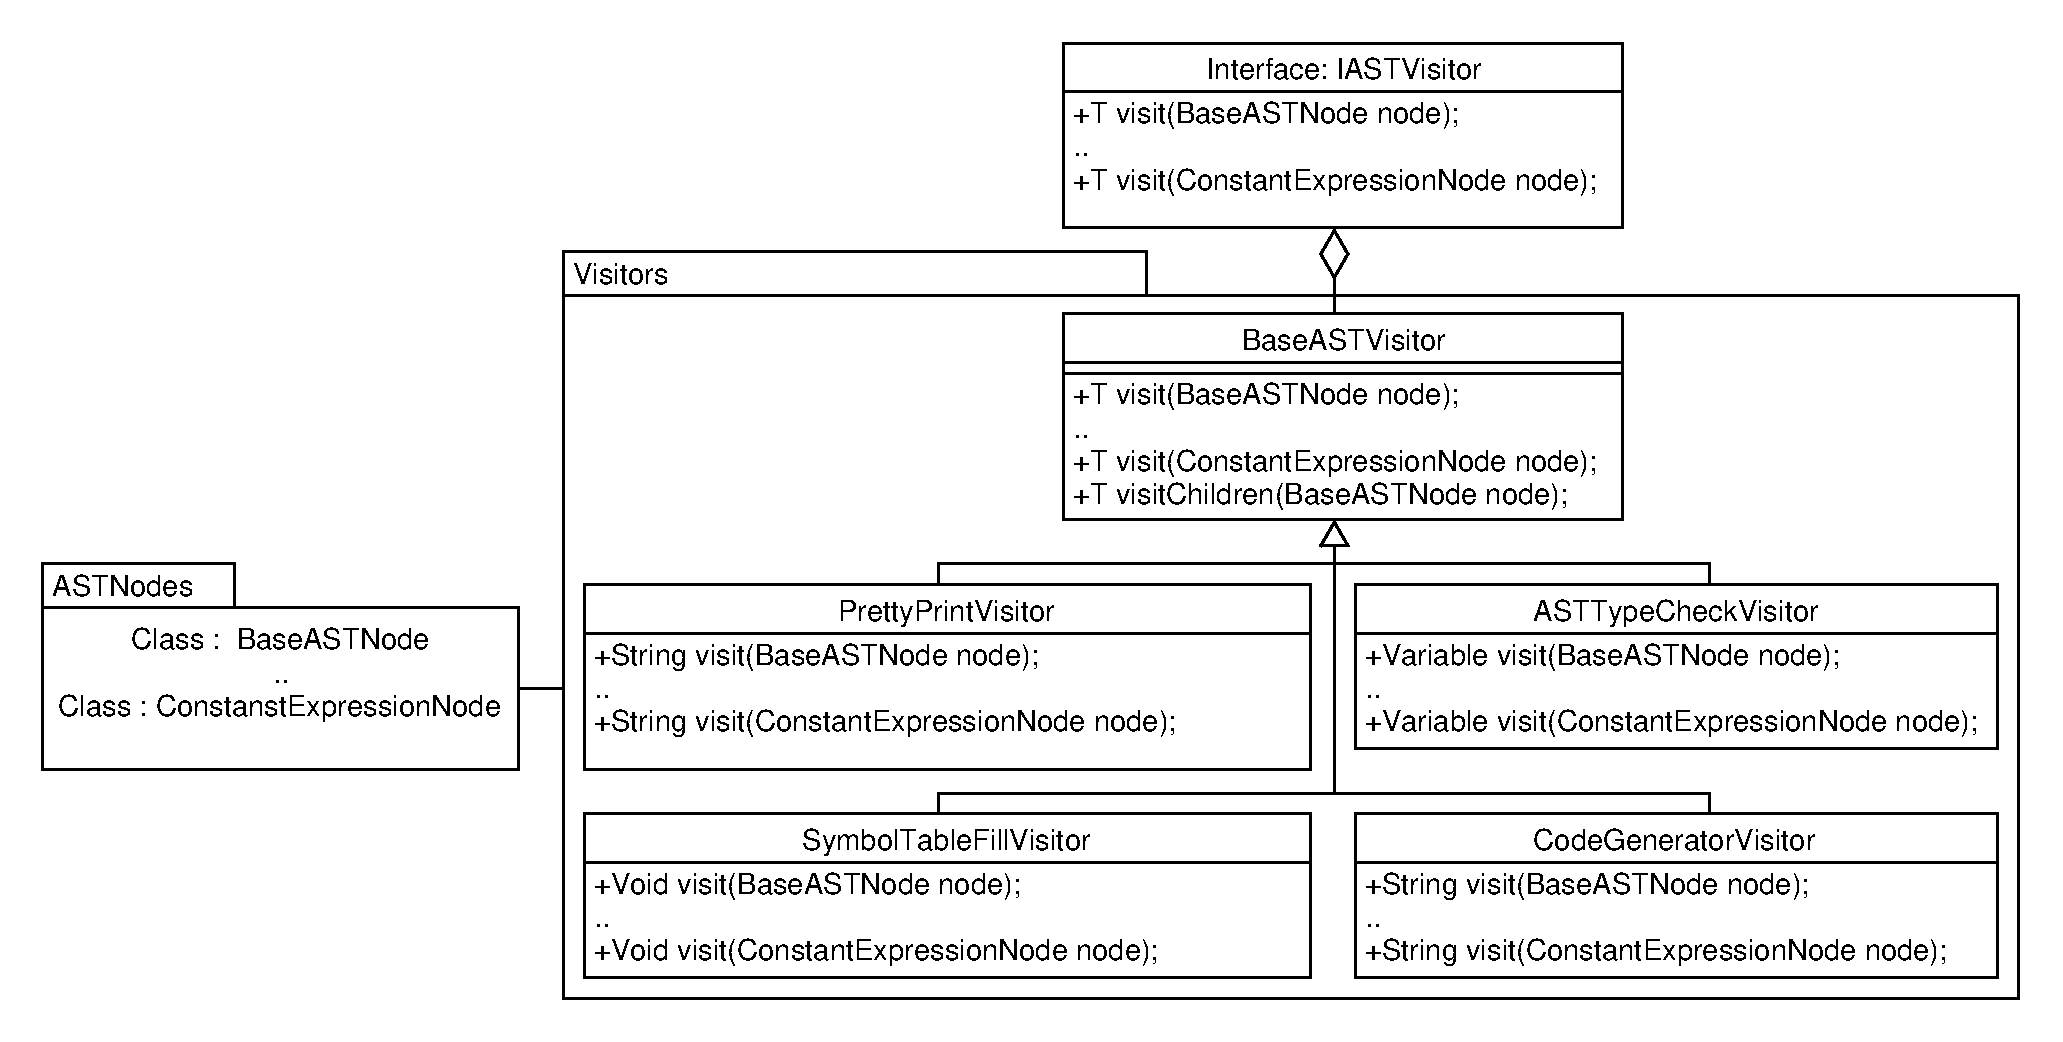
\includegraphics[width=1\textwidth]{figures/ClassDiagrams/Visitors.pdf} % trim=4.85cm 15cm 0.85cm 1cm
\caption{A UML diagram of the visitor patterns implementation in the compiler for traversing the \acrshort{ast}.}\label{image:Visitors}
\vspace{-15pt}
\end{figure} 